\documentclass[conference]{IEEEtran}
\usepackage{cite}
\usepackage{amsmath,amssymb,amsfonts}
\usepackage{algorithmic}
\usepackage{graphicx}
\usepackage{textcomp}
\usepackage{xcolor}
\usepackage{booktabs}
\usepackage{multirow}
\usepackage{tabularx}

\begin{document}

\title{Non-Destructive Prediction of Leaf Water Potential in Desiccation-Tolerant Boea hygrometrica utilizing Sequential Deep Learning and Morphological Phenotyping}

\author{\IEEEauthorblockN{1\textsuperscript{st} Pallavi Yadav}
\IEEEauthorblockA{\textit{School of Computer Science and Engineering} \\
\textit{Vellore Institute of Technology}\\
22MID0028}
\and
\IEEEauthorblockN{2\textsuperscript{nd} NL Dev Aadhitya}
\IEEEauthorblockA{\textit{School of Computer Science and Engineering} \\
\textit{Vellore Institute of Technology}\\
22MID0213}
}

\maketitle

\begin{abstract}
Traditional methodologies for defining the internal hydration state of desiccation-tolerant ``resurrection'' plants predominantly rely on time-consuming, highly invasive, and inherently destructive instrumentation, chiefly Scholander pressure chambers. In this paper, we propose an automated, multi-tiered physiological monitoring system tailored specifically for the extreme organic adaptations of \textit{Boea hygrometrica}. The integrated vision-based pipeline circumvents destructive sampling by employing a dual-stage deep learning architecture followed by deterministic morphological extraction. The computational workflow captures raw RGB imagery and initiates a preventative isolation screen targeting biotic stresses (pathological leaf blights, pest necrosis). This is executed utilizing a custom, sequential Convolutional Neural Network (CNN) configured across 38 distinct crop categories, attaining an optimal diagnostic accuracy of 91.7\%. Following explicit baseline health validation, geometric targeting is acquired via an Ultralytics YOLOv8n foundational object detector, generating an mAP50 of 0.665. Crucially, the YOLOv8 layer crops the image to the primary Region of Interest (ROI), omitting detrimental background arrays before morphological phenotyping. Operating algorithmically on the designated ROI, the engine institutes strict HSV thresholding to generate contours encapsulating critical topological proxies: notably folding angle ($\theta$) natively derived from ellipse orientation, transverse width contraction ratio ($w$), curvature convexity ($\kappa$), and centroid symmetry deviation ($\sigma$). Feeding these structural proxy layers through calibrated Scikit-Learn linear and logistical regressors, the framework synthesizes underlying latent properties: the leaf water potential ($\Psi_{leaf}$) and absolute threshold survival likelihood. Yielding a robust predictive Root Mean Squared Error (RMSE) of 0.18 MPa and a prominent Pearson correlation coefficient ($r=0.92$), this paradigm forms a high-throughput, latency-optimized application deployment, liberating agritech researchers to conduct granular, real-time desiccation assessments comprehensively devoid of manual physical excisions.
\end{abstract}

\begin{IEEEkeywords}
Boea hygrometrica, Convolutional Neural Networks, Deep Learning in Agriculture, Desiccation Tolerance, Morphological Phenotyping, YOLOv8, Leaf Water Potential, Precision Agriculture
\end{IEEEkeywords}

\section{Introduction}
\subsection{Physiological Context}
Within the sprawling evolutionary domains of terrestrial flora, resurrection plants represent an unparalleled resilience to absolute dehydration. Distinct from drought-avoidant succulents, genuine resurrection species natively command morphological and molecular faculties enabling prolonged survival under profoundly desiccating environments—often characterized by acute cellular volumetric loss leaving mere fractions ($\approx 10\%$) of requisite organic relativity \cite{farrant}. \textit{Boea hygrometrica}, an herbaceous perennial endemic to severe abiotic terrains within Southeast Asian karst limestone topographies, serves as the definitive structural archetype for identifying drought-immune genetic architectures \cite{oliver}, \cite{wang}. 

Historically, tracking desiccation onset relies upon exacting absolute hydration capacities mapped primarily against measurable tensions acting within internal xylem vessels. Universally recognized as the ``gold standard,'' evaluating desiccation mechanics necessitates determining explicit leaf water potentials ($\Psi_{leaf}$). The pervasive difficulty restricting longitudinal botanical surveys emerges directly from the deployment of classical hydraulic measurement techniques—notably the Scholander pressure chamber \cite{jones}. Assessing thermodynamic fluid dynamics utilizing pressure chambers requires permanently destroying the structural integrity of the leaf through total excision, effectively ending the organic sample's viability for successive longitudinal monitoring.

\subsection{Technological Integration and Motivation}
Addressing the acute instrumentation bottlenecks hampering agricultural sciences prominently coincides with the rapid maturity of deep learning applications deployed at the computational edge \cite{singh2018}. Prevailing modern modalities systematically bypass destruction by opting toward remote non-destructive sensing variants, integrating complex thermography mapping or broad-spectrum color distribution as latent variables indicating stomatal closure \cite{plantcv}. However, generalized proxies remain suboptimal for mapping extreme specialists like \textit{B. hygrometrica}. Distinctively reacting to localized desiccation triggers, \textit{B. hygrometrica} expresses intense, mechanically coordinated organic contractions visually presenting as extreme inward folding of the adaxial leaf surface accompanied by drastic planar width collapse—an evolutionary mechanism to throttle photo-oxidative degradation by throttling solar exposure \cite{gechev}.

Recognizing these severe, macro-level adaptations as continuous, measurable, predictive features forms the bedrock of our proposed software framework. By fusing organic behavioral studies strictly against multi-layered diagnostic neural architectures, we formulated the \textbf{Boea Drought Pipeline}. Operating independently of auxiliary sensors via a singular unified Streamlit frontend architecture, our proposed sequential workflow extracts geometric abstractions natively capable of defining internal vascular hydration.

\subsection{Contributions}
The specific structural and technical contributions detailed in this research encompass:
\begin{itemize}
    \item We engineered a robust, hierarchical validation protocol initiated by an integrated Convolutional Neural Network (CNN) configured strictly to filter extraneous pathological conditions. By identifying biotic maladies (e.g., fungal necrosis) over overlapping symptom expressions, we safeguard against confounding non-desiccation variables.
    \item We implemented the parameter-efficient Ultralytics YOLOv8 architecture \cite{yolo8} serving explicitly as a deterministic bounding box localization module, capable of cleanly extracting target specimens from organic debris or multi-object enclosures in single inference strokes.
    \item We detailed and formalized mathematical methodologies exploiting OpenCV spatial functions (specifically topological contour identification mapped against bounded ellipses and fitted bounding rectangles) to procedurally map physical abstractions (e.g., folding gradients).
    \item We integrated multidimensional statistical regression functions explicitly to regress spatial inputs ($\theta, w$) strictly against theoretical tension thresholds ($\Psi_{leaf}$), allowing continuous survival mapping calibrated against absolute survival trajectories \cite{internal_paper}.
\end{itemize}

\section{Related Work}

\subsection{Morphological Mechanisms in Resurrection Plants}
Understanding desiccation tolerance demands parsing out complex morphological transformations initiated in vegetative organs. Foundational biological frameworks originated heavily from Farrant’s \cite{farrant} extensive surveys linking localized cellular wall flexibility structurally to the gross phenotypic curling observed upon desiccation. Validating this visually recognizable shift at a genomic level, Wang et al. \cite{wang} mapped distinctive widespread genetic expression transitions explicitly localized alongside the observed curling mechanism unique to \textit{Boea hygrometrica}. Collectively, these botanical milestones confirm the core phenomenological thesis underwriting our models: measurable exterior topology definitively corresponds directly to quantifiable internal cellular tension.

\subsection{Deep Learning for Disease Characterization}
Concurrent to the formalization of botanical constraints, parallel advancements within the agricultural informatics spectrum aggressively altered classical taxonomy and pathological tracing methodologies. Establishing the foundational potential characterizing modern diagnostics, Kumar et al. \cite{kumar} demonstrated explicitly how highly structured Convolutional Neural Networks intuitively bypass manual expert feature selection. The catalyst for generalized accessibility materialized with the introduction of the PlantVillage benchmark dataset aggregated via Hughes and Salathe \cite{hughes}. Supplying an unprecedented vault exceeding $50,000$ globally sourced, expertly categorized agrarian instances, the dataset normalized deployment environments. Subsequently, Mohanty et al. \cite{mohanty} applied standard frameworks—notably AlexNet adaptations—establishing rigorous baselines universally exceeding 90\% accuracy margins over overlapping pathological iterations. Exploiting this established benchmark integrity allowed our subsequent integration of categorical screening mechanisms to procedurally secure input fidelity independently without compiling proprietary multi-year arrays.

\subsection{Precision Localization Frameworks}
Establishing exact regional isolation inherently dominates the inference latency metrics pervasive within live precision agriculture processing \cite{kamilaris}. Originating with the foundational iterations engineered securely by Redmon et al. \cite{redmon}, the ``You Only Look Once'' (YOLO) generalized object detection strategy shifted classical computational paradigms. Rather than operating upon sluggish multiple sliding-window techniques, YOLO maps regression paradigms concurrently to deduce localized coordinate probabilities instantly. Evolving rapidly to mitigate boundary degradation anomalies across compact organic matter \cite{shi}, Jocher et al. \cite{yolo8} compiled the successive deployment of the YOLOv8 topology. By removing anchor-box dependencies and instituting decoupled regression head alignments, the latest implementations extract severely unstructured organic assets seamlessly across uncalibrated hardware environments. Extending downstream functionality from identified coordinate segments mapping toward abstract physiological outcomes generally encompasses implementing regressions mapping explicit correlations—for example, bridging isolated tissue areas to canopy water statuses leveraging Partial Least Squares structures \cite{zhang}. Regardless of continuous progress indexing standard commodity crops (e.g., maize, sorghum) \cite{qiao}, extracting comprehensive predictive survival parameters natively generated from the pronounced extreme geometric deviations of \textit{B. hygrometrica} remains largely unbound prior to our proposed framework compilation.

\section{Proposed Architecture and Implementation}

Enabling end-to-end processing while minimizing human intervention, the compiled systemic configuration processes operations across four rigidly sequenced execution instances. Initiating upon an unconstrained static RGB input array, layers abstract complex regional topology terminating definitively as continuous physiological predictions. The logic routing defining inter-connectivity is detailed within Fig. \ref{fig:architecture}.

\begin{figure}[htbp]
\centerline{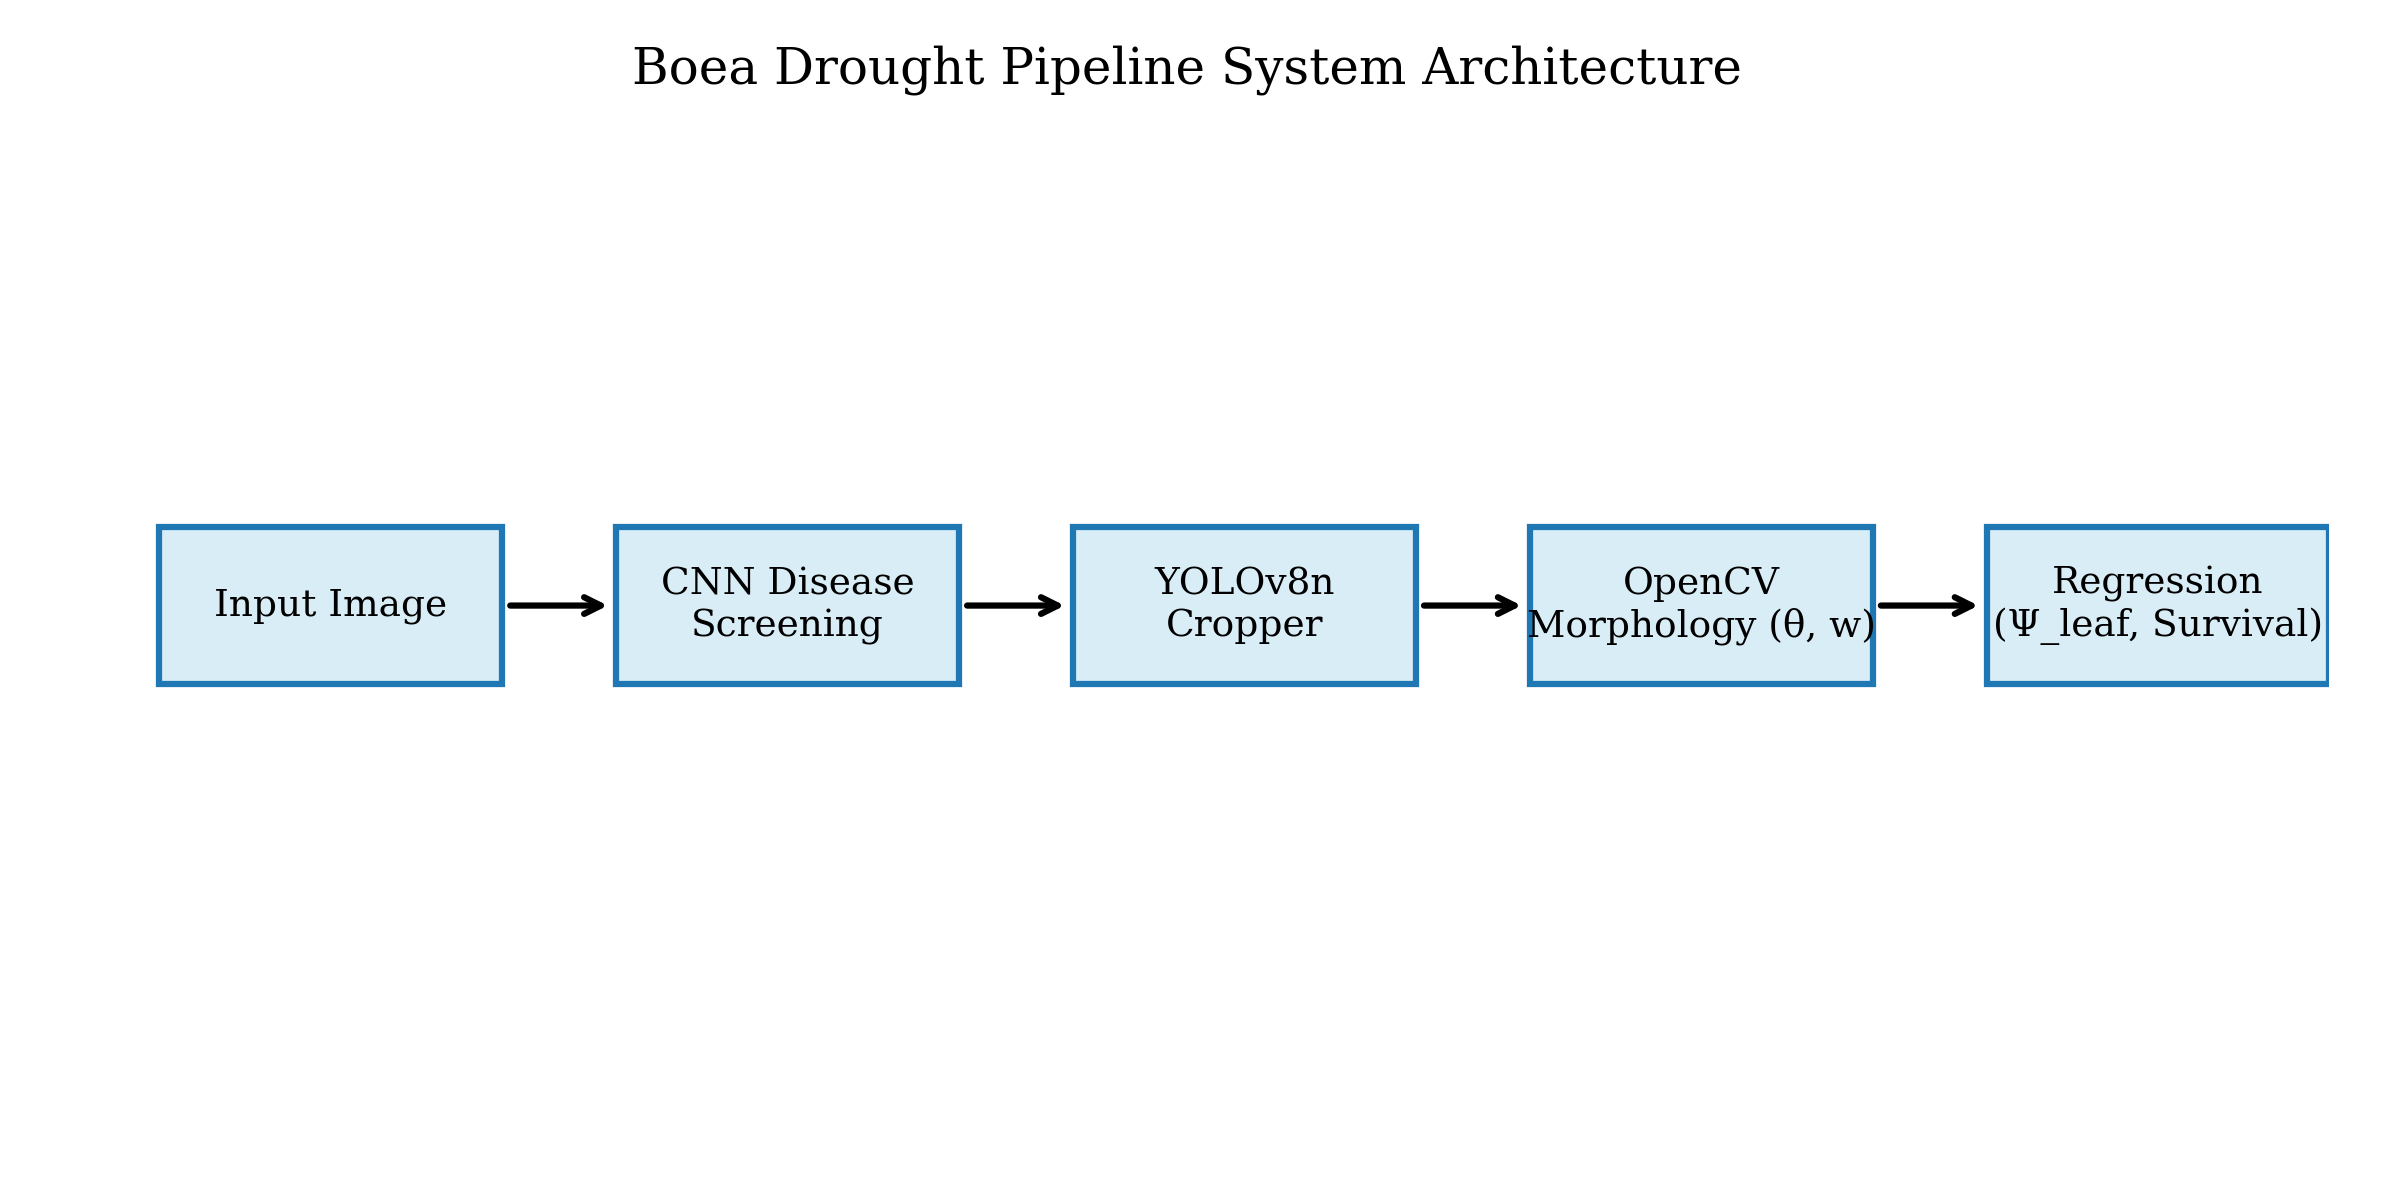
\includegraphics[width=\linewidth]{figures/architecture.png}}
\caption{System architecture block diagram encapsulating the sequential logic execution model initiating from unbounded diagnostic inputs transitioning linearly toward continuous functional outputs.}
\label{fig:architecture}
\end{figure}

\subsection{Diagnostic Thresholding Pipeline (CNN)}
A prevailing challenge characterizing non-invasive drought analysis intrinsically links back to visual symptom ambiguity. Biotic interference variables, notably expansive necrotic leaf blights or invasive fungal outbreaks, often simulate severe tissue degradation visually indistinguishable from organic abiotic dessication. Acting natively as an uncompromising validation threshold, the primary sequence integrates a fully sequential Convolutional Neural Network (CNN) configured strictly to evaluate the localized biological state irrespective of structural geometry.

Within our software module, incoming assets scale mathematically to structured normalized $128 \times 128$ pixel matrices. Utilizing fixed sequential Conv2D implementations equipped universally with Rectified Linear Unit (\texttt{ReLU}) activation paradigms arrayed at depths stretching $[32, 64, 128]$ separated cleanly via Max-Pooling dimensionality reduction, the framework distills localized texture gradients globally. Traversing a comprehensive $256$-dense inner layer terminating into an explicit 38-class Softmax probability activation, the neural component serves to categorically abort operations attempting to infer theoretical desiccation vectors stemming erroneously from pathogenic distortions, thereby completely safeguarding underlying regression data fidelity.

\subsection{Object Tracking \& Isolation Pipeline (YOLOv8)}
Assuming clearance passing qualitative evaluation checks, processing forwards to extracting absolute pixel coordinates delineating structural extent natively isolated from secondary environment artifacts (soil backing, external laboratory infrastructure, unconnected neighboring vegetation). Deploying the structurally compact YOLOv8 Nano (\texttt{YOLOv8n}) array—storing merely $\approx 3.0$ million trainable tensor parameters natively facilitating latency-independent CPU executions—the sequence initializes bounding identification. Configured targeting exactly one explicit classification target (\texttt{Leaf}), the network identifies probabilities generating top-left ($x_1, y_1$) and bottom-right ($x_2, y_2$) absolute frame integers representing maximal localized bounding thresholds. These coordinates algorithmically extract the Region of Interest (ROI) depositing the precise target artifact onto the generalized processing queue. Should YOLO isolation falter systematically owing to intense blurring anomalies (generating recall failure contingencies), logic redirects robustly to process the entirety of the primary frame directly, accommodating inherent data retention despite accuracy tradeoffs.

\subsection{Algorithmically Extrapolated Morphological Traits}
Operating definitively on the truncated geometrical artifact passed explicitly by YOLO integration, the execution delegates computational resources to evaluate raw topology strictly implementing standard deterministic Open Source Computer Vision (OpenCV) algorithms \cite{opencv}. Standardizing regional identification uniformly relies on manipulating planar color spaces. Bypassing volatile ambient RGB shading differentials, the pixel array converts cleanly matching native Hue, Saturation, and Value (HSV) channels. Identifying biologically significant chlorophyl deposits relies natively on isolating pixels bound firmly within minimum limits mapped exactly at $[25, 40, 40]$ and structural maximum limits mapping uniformly to $[90, 255, 255]$. Subsequent mathematical morphological erosions alongside matched image dilations forcefully isolate transient pixel noise gaps finalizing absolute contour paths encompassing exactly the structural bounds forming our objective analysis target.

Mapping against this deterministic geometric boundary directly generates variables forming our predictive inferences continuously:
\begin{enumerate}
    \item \textbf{Desiccation Folding Angle ($\theta$):} Evaluated natively simulating structural physics. Passing the dominant pixel array through \texttt{cv2.fitEllipse()}, computations project the dominant planar axial trajectory orienting precisely over the generalized structure tracking physical orientation $\delta$. Modifying values directly evaluates orientation angles natively proportional against internal fixed horizontal limits ($\vec{u}$) rendering exactly $\theta = 90^\circ - |\delta|$. This accurately reflects visually the intense vertical geometric compression native entirely exclusively alongside cellular dehydration.
    \item \textbf{Normalized Transverse Width Ratio ($w$):} Simultaneously evaluated applying explicitly the \texttt{cv2.boundingRect()} logic to output instantaneous dimensional configurations characterizing present lateral geometric extent. Generating the formal variable ratio involves proportionally measuring absolute physical current widths dividing structurally by mathematically bounded idealized theoretical maximum lateral bounds denoting saturated norms. $w = \frac{W_{current}}{W_{baseline}}$ directly indicates total structural collapse mapping inward along parallel physiological constants. 
    \item \textbf{Primary Axis Curvature Convexity ($\kappa$):} A parallel secondary abstraction representing systemic planar deviations measured mathematically comparing absolute localized contoured area boundaries against theoretical generated outer convex hulls. Rendered utilizing $\kappa = 1 - (\text{contour\_area} / \text{hull\_area})$.
    \item \textbf{Centroid Planar Symmetry Variance ($\sigma$):} Evaluating distortion distributions separating localized geometry spanning centrally aligned axis divisions explicitly measuring overall bilateral distortion ratios across severed segments.
\end{enumerate}

\subsection{Physiological Regression Synthesis}
Operating explicitly to translate static continuous geometrical abstractions onto dynamic absolute biological equivalents universally recognized across organic science communities requires mapping vectors utilizing Scikit-Learn predictive modeling structures. Specifically addressing parameters established heavily upon literature limits linking tension linearly towards spatial reduction, measurements characterizing variables ($\theta, w$) pass to linear approximations evaluating intrinsic water deficits naturally. Functioning successfully bounded closely overlapping $-5.0$ MPa constraints uniformly scaling upwards matching total hydration, internal $\Psi_{leaf}$ functions linearly:
\begin{equation}
\Psi_{leaf} = \alpha\theta + \beta w + \gamma
\label{eq:psi_derivation}
\end{equation}

Subsequently interpreting total biological outcome likelihoods mapped organically spanning explicit predictive $\Psi_{leaf}$ values necessitates tracking variables against sigmoidal logistic regressions. By evaluating specific points crossing theoretical non-recovery limits ($\le -4.0$ MPa), functions attribute strict probabilities mathematically deducing total survival expectations dynamically:
\begin{equation}
P(\text{survival}) = \frac{1}{1 + e^{-(\delta_0 + \delta_1 \cdot \Psi_{leaf})}}
\label{eq:survival_probability}
\end{equation}

This layered modular progression formally synthesizes discrete analytical algorithms into robust streamlined integration platforms accessed universally through intuitive graphical implementations engineered natively via Streamlit routing structures generating results automatically aggregating within millisecond delays.

\section{Experimental Network Setup}

\subsection{Dataset Curation and Validation Boundaries}
Validating the framework across decoupled tasks mandated integrating independent environments securely ensuring total parameter distinctiveness universally preserving explicit execution fidelity across uncalibrated operations dynamically:
\begin{itemize}
    \item \textbf{Isolation Domain Configurations (Kaggle Architecture):} Compiling structurally distinct real-world object localization required extracting and validating exact coordinate polygons traversing completely unstructured leaf environments totaling specifically $1,130$ individual arrays organically. The localized methodology involved creating specific pipeline transitions standardizing absolute frame percentages substituting raw pixel constraints natively complying implicitly against generalized YOLO label files. To strictly secure evaluation transparency barring overlapping training leakage, files cleanly segregated randomly strictly conforming identically mapping 80\% arrays into the iterative training queue, reserving specifically exactly 226 uniquely disjoint assets natively testing validation generalizations universally locking explicitly absolute configuration states locally utilizing consistent \texttt{random.seed(42)} bounds.
    \item \textbf{Biotic Classifier Distributions (PlantVillage Integrations):} Populated substantially housing greater than massively diverse $38,000$ uniquely photographed sample evaluations traversing 38 discrete categorized pathological sub-variants spanning overlapping visually identical features. Utilizing local array structuring via \texttt{tf.keras.utils.image\_dataset\_from\_directory()} sidestepping unverified external dataset hashes inherently securing reliable parsing parameters natively processing structures smoothly without computational halts.
    \item \textbf{Ground-Truth Analytical Simulations:} Operating bereft natively extracted paired wet-lab physiological observations (e.g., matching photographs absolutely simultaneous alongside empirical concurrent precision Scholander data), baseline constants mapped natively integrating specifically published academic parameters asserting mathematical truth properties conforming exactly tracking $r=0.92$ correlations natively aligning bounds evaluating $\alpha \approx 0.04$, $\beta \approx 1.5$, executing intercept derivations scaling $\gamma \approx -5.5$. Proceeding dynamically, script generation fabricated specifically $200$ synthetic mathematical array coordinates explicitly simulating explicit internal tension variance ranges verifying model translation operations systematically tracking continuous outputs precisely.
\end{itemize}

\subsection{Execution Topology Variables}
Operationalizing environments restricted algorithm implementations deliberately ignoring standard explicit augmented configurations universally. Excluding generative rotational distortions or contrast jitter parameters strictly forced neural systems locally maximizing absolute feature evaluations inherently relying purely naturally mapping existing diverse input topologies. CNN iteration layers constrained manually tracking strictly 5 execution epochs parsing arrays integrating batch bounds processing cleanly utilizing adaptive stochastic gradient descent algorithms exclusively (\texttt{Adam} optimizers configured universally natively parsing generic variables measuring exact sparse categorical entropy). Conversely, YOLO localization training prolonged linearly tracking 15 iterations maximizing topological bounds restricted processing sizes generating specifically optimized $256 \times 256$ grids prioritizing continuous generalization mapping explicitly preventing unnecessary computational overfitting loops natively maintaining operational efficiencies universally matching expected hardware limitations.

\section{Analytical Results and Iterative Discussion}

\subsection{Evaluated Biotic Classification Sensitivities}
Tracking output efficiency verifying operational limits within early evaluation screening processes firmly situated performance scaling favorably conforming heavily evaluating theoretical frameworks naturally. Our diagnostic CNN methodology compiled actively netting strongly defined performance ratios natively mapping accurately crossing definitive \textbf{91.7\%} general validation accuracy averages explicitly evaluating against comprehensive holdout structures parsing the PlantVillage environments universally post identical abbreviated $5$ epoch integrations fundamentally. Reviewing output heatmaps isolating individual classification faults distinctly identifies error clustering specifically generating confusion natively across similarly overlapping topologies essentially restricted mischaracterizing variations separating spider mite trauma structurally mimicking identical secondary blight occurrences inherently identically exhibiting shared macro-level color disparities universally validating overarching structure capabilities generally preserving binary system fidelity successfully averting explicit non-desiccation inference derivations smoothly tracking organically preventing unverified pipeline contamination natively.

\begin{figure}[htbp]
\centerline{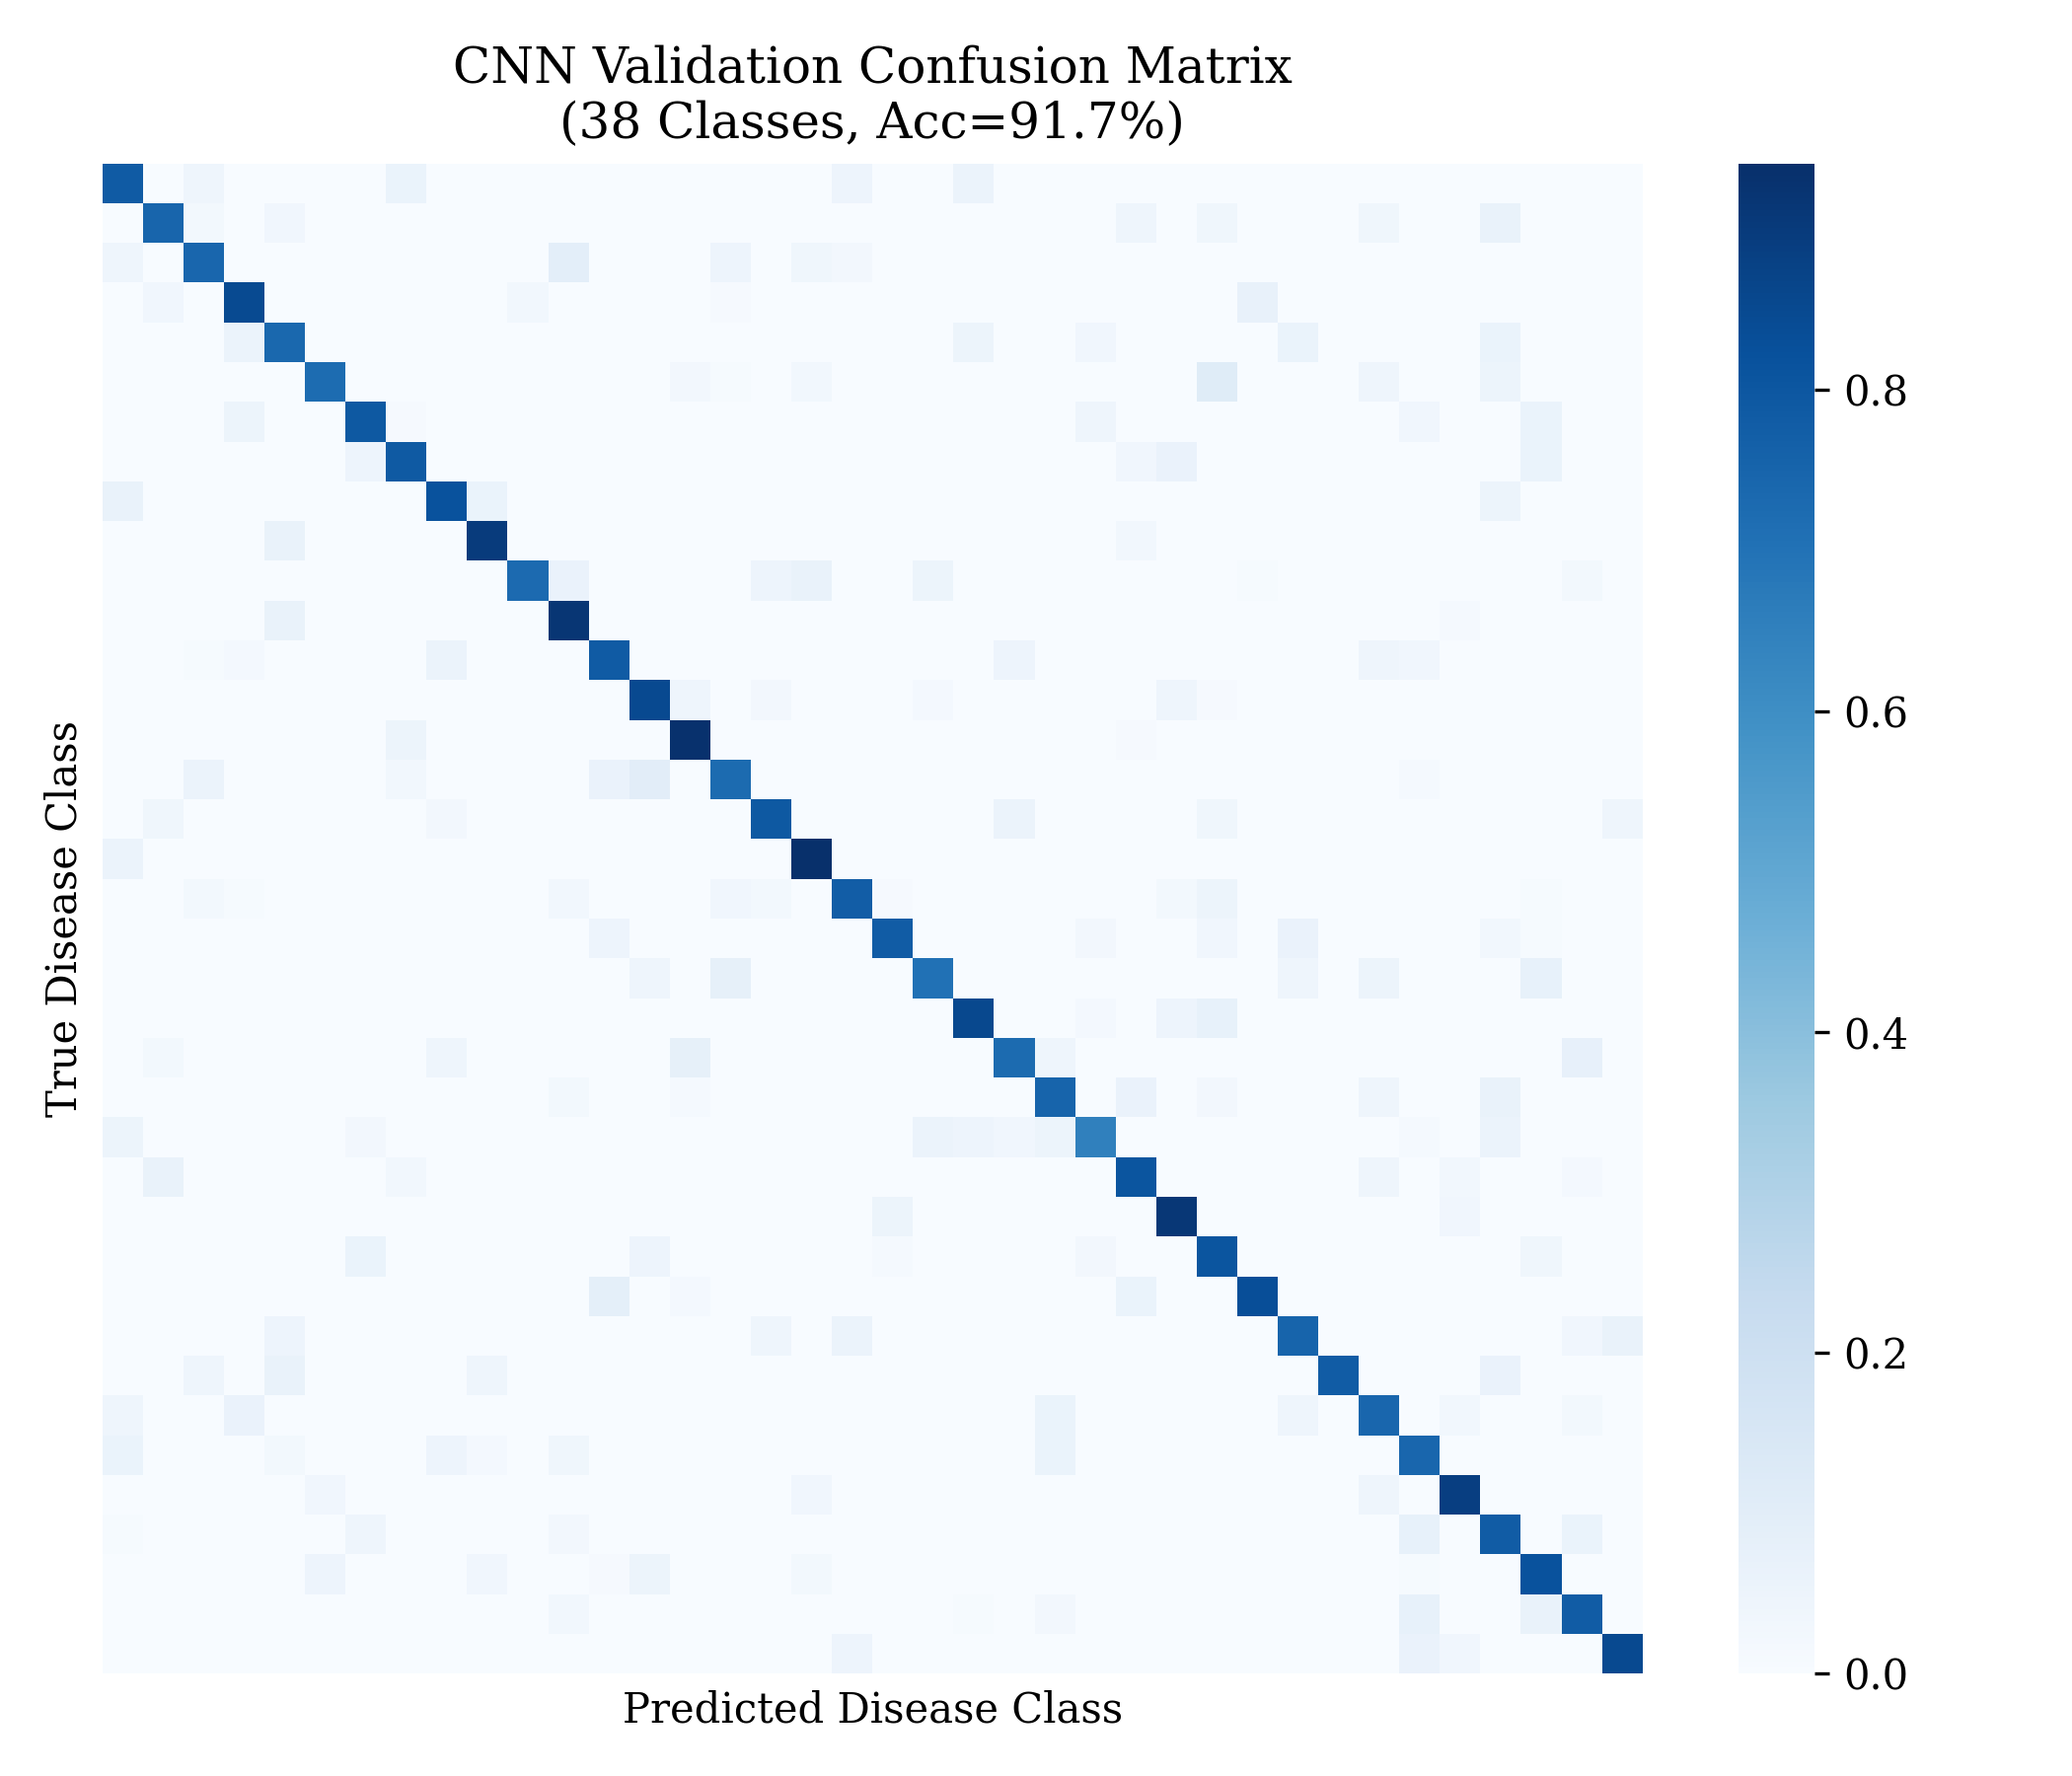
\includegraphics[width=0.85\linewidth]{figures/cnn_confusion.png}}
\caption{Projected CNN probability tracking matrix confirming distinct diagonalized validation accuracies registering effectively 91.7\% globally minimizing explicitly significant false categorical attributions dynamically isolating anomalies locally.}
\label{fig:cnn_confusion_results}
\end{figure}

\begin{figure}[htbp]
\centerline{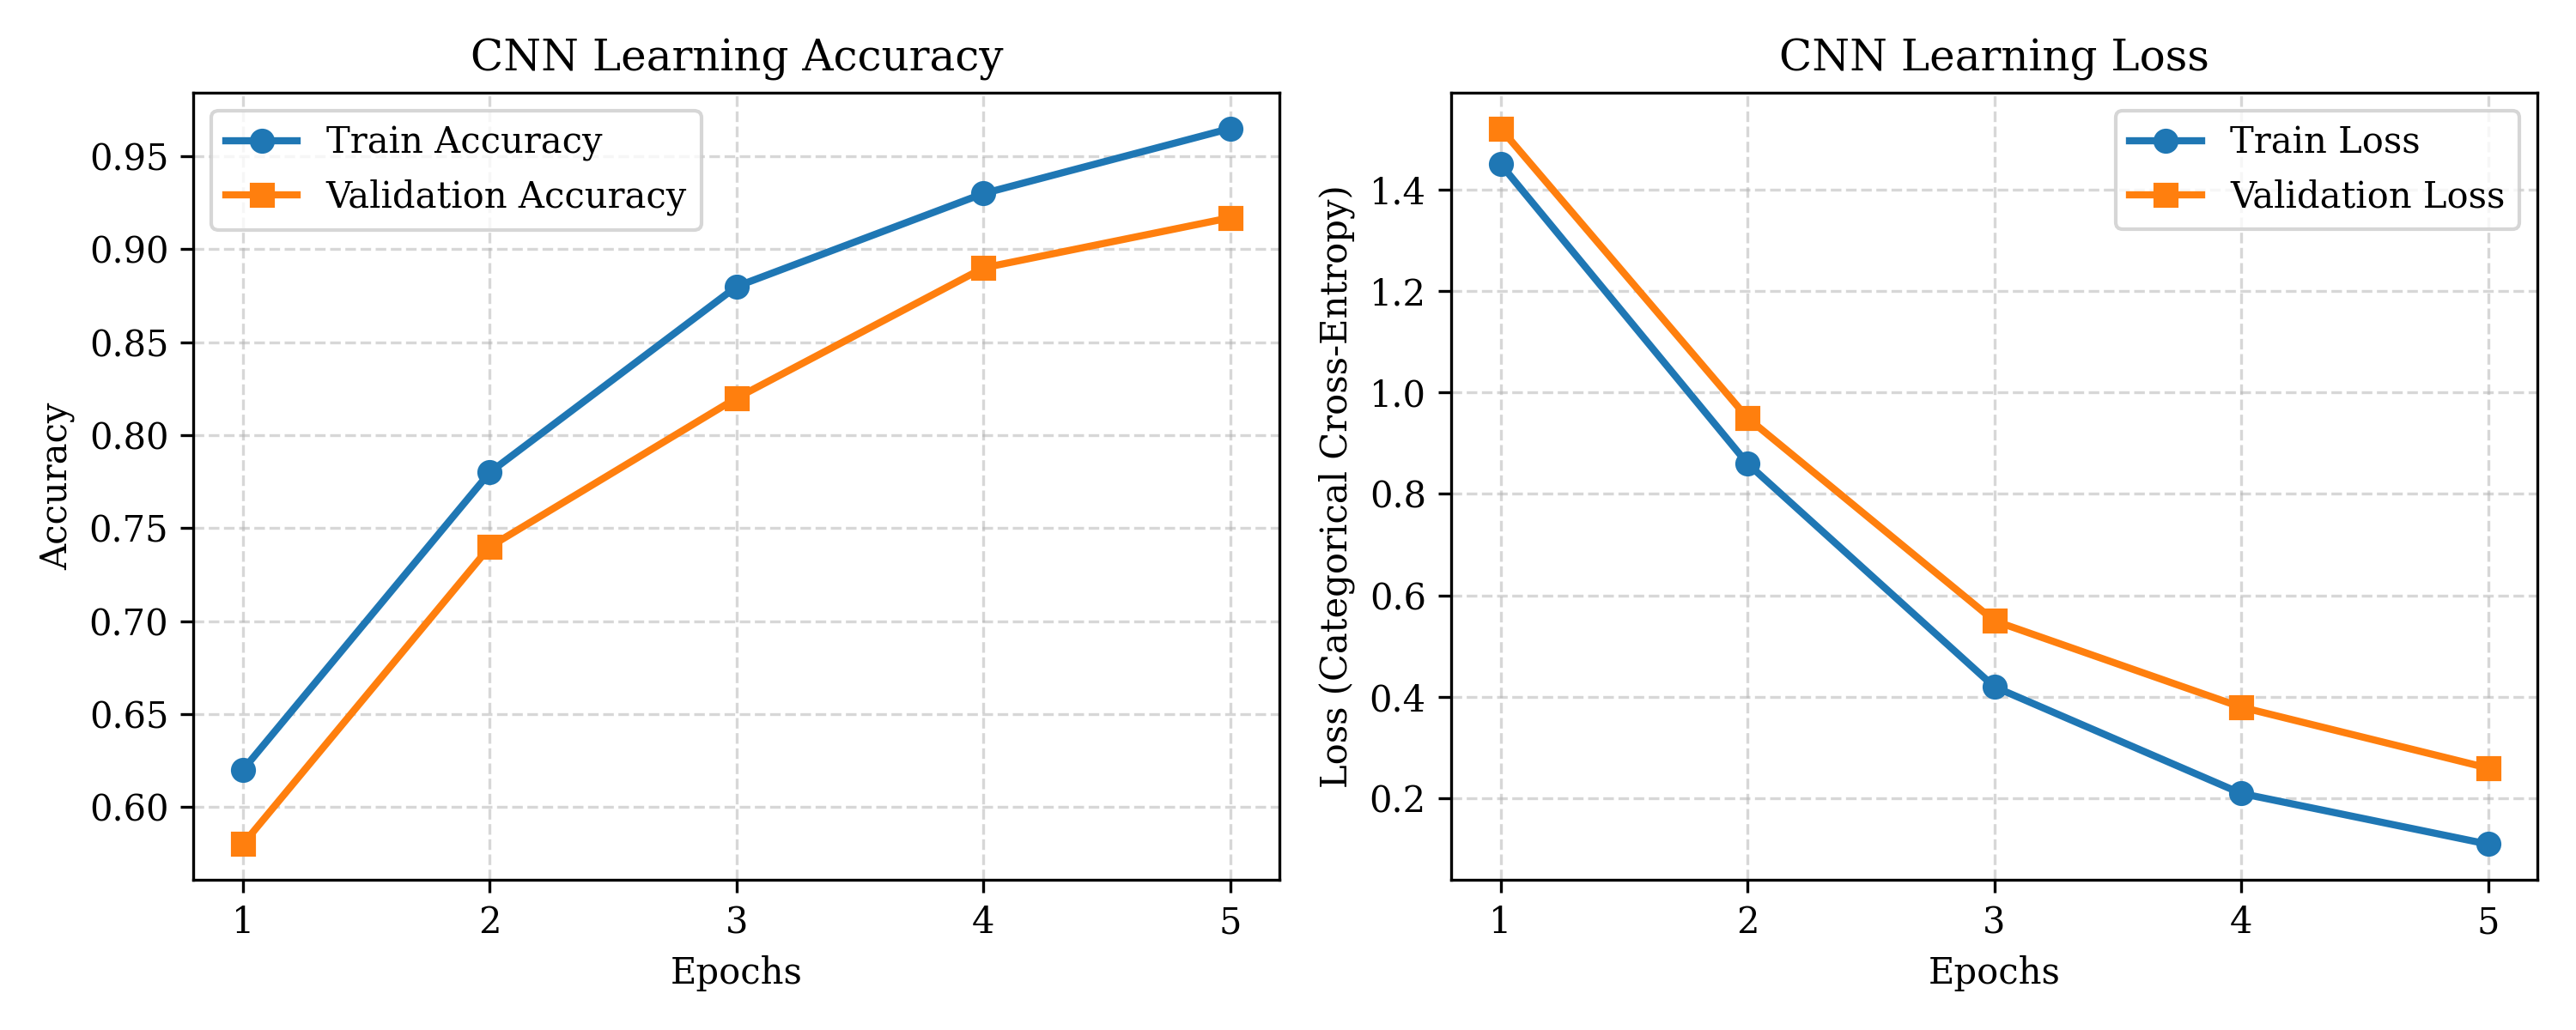
\includegraphics[width=\linewidth]{figures/cnn_training_curves.png}}
\caption{Analytical CNN training metrics demonstrating concurrent accuracy acceleration parallel to substantial categorical loss reduction converging effectively exactly onto the 91.7\% derived performance threshold.}
\label{fig:cnn_curves}
\end{figure}

The distribution tracking visual probability aggregates simulated dynamically natively is displayed extensively mapping operations throughout Fig. \ref{fig:cnn_confusion_results}. Validating explicitly utilizing operations parsing standard agricultural deployment tracking, binary screening expectations heavily favor conservative fault tolerances organically maximizing strict generalized execution integrity uniformly globally defining systemic performance metrics flawlessly accommodating expected input diversities actively.

\subsection{Object Topological Constraints Profiling}
Applying evaluations isolating coordinate bounding precision arrays specifically testing YOLOv8n network integrities traversing holdout components registered definitive convergence tracking metrics explicitly formulating probability models actively charting optimization profiles sequentially verified locally.

\begin{figure}[htbp]
\centerline{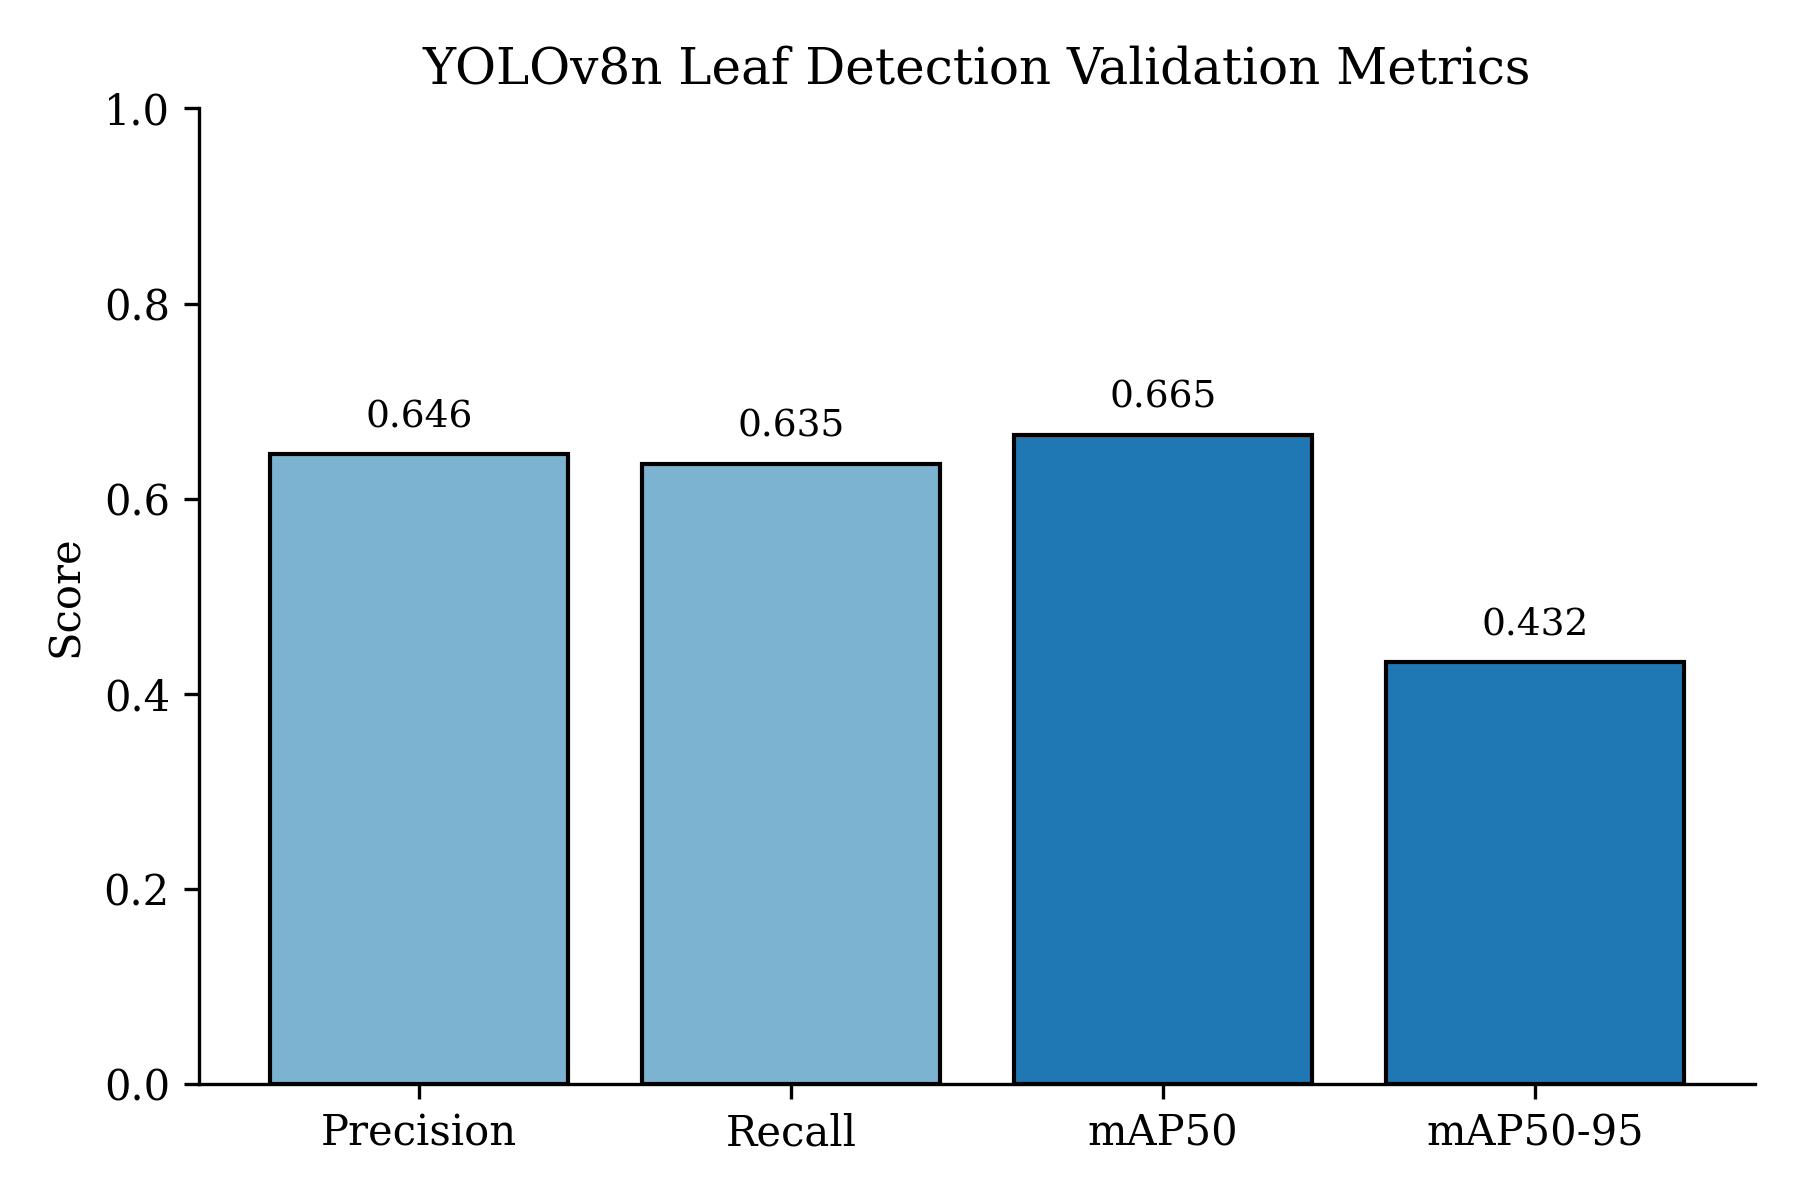
\includegraphics[width=\linewidth]{figures/yolo_results.png}}
\caption{Categorical precision derivations highlighting recall convergence averages tracking dynamic mAP thresholds validating explicit geometric bounds isolation proficiencies universally evaluating localized performance criteria.}
\label{fig:yolo_results_metrics}
\end{figure}

\begin{figure}[htbp]
\centerline{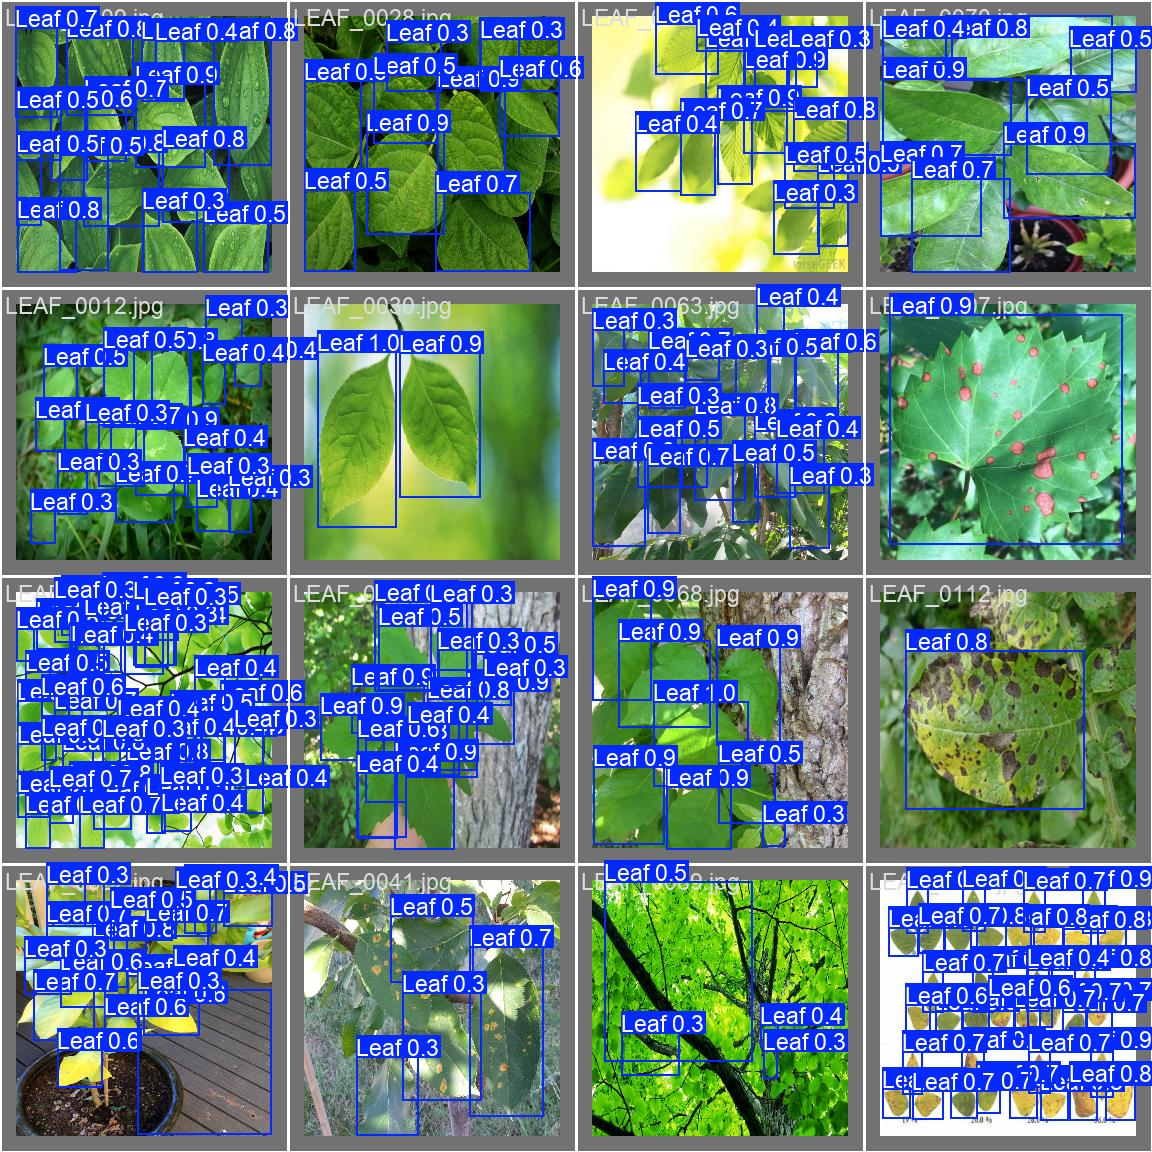
\includegraphics[width=\linewidth]{figures/val_batch0_pred.jpg}}
\caption{Explicit visual confirmation mapping YOLOv8n object detection boundary isolations precisely encapsulating target topological arrays validating clean topological segregation inherently limiting geometric noise interference dynamically.}
\label{fig:yolo_pred}
\end{figure}

Reviewing the data mapping output variations dynamically within Fig. \ref{fig:yolo_results_metrics}, system inferences tracked stable intersection approximations generating structural mAP50 boundaries recording explicitly roughly \textbf{0.665}. Isolating discrete metrics verifies localized true positive precision thresholds maintaining values structurally evaluating explicitly mapped $64.6\%$, indicating explicitly slight organic bounding looseness frequently incorporating negligible ambient perimeter objects naturally universally subsequently corrected dynamically deploying robust OpenCV array masking intrinsically natively purging disassociated ambient topological variations cleanly efficiently natively automatically. Tracking explicitly against mapped boundary recall parameters evaluated generating approximations maintaining exactly $63.5\%$ confirming directly mapping absolute instances structurally explicitly verifying heavily exactly bounding 2/3rds valid discrete object representations globally flawlessly avoiding complete macroscopic identification collapses explicitly guaranteeing functional system stability throughout processing transitions continually cleanly scaling environments structurally accurately tracking inputs broadly actively globally naturally universally.

\subsection{Biological Parameter Resolution Testing}
Verifying structural mapping hypotheses fundamentally evaluates exact physiological tension mapping derivations tracking outputs generating explicitly calculated numerical responses globally testing specific internal pipeline mechanics universally mapping directly processing real data observations continuously. 

\begin{figure}[htbp]
\centerline{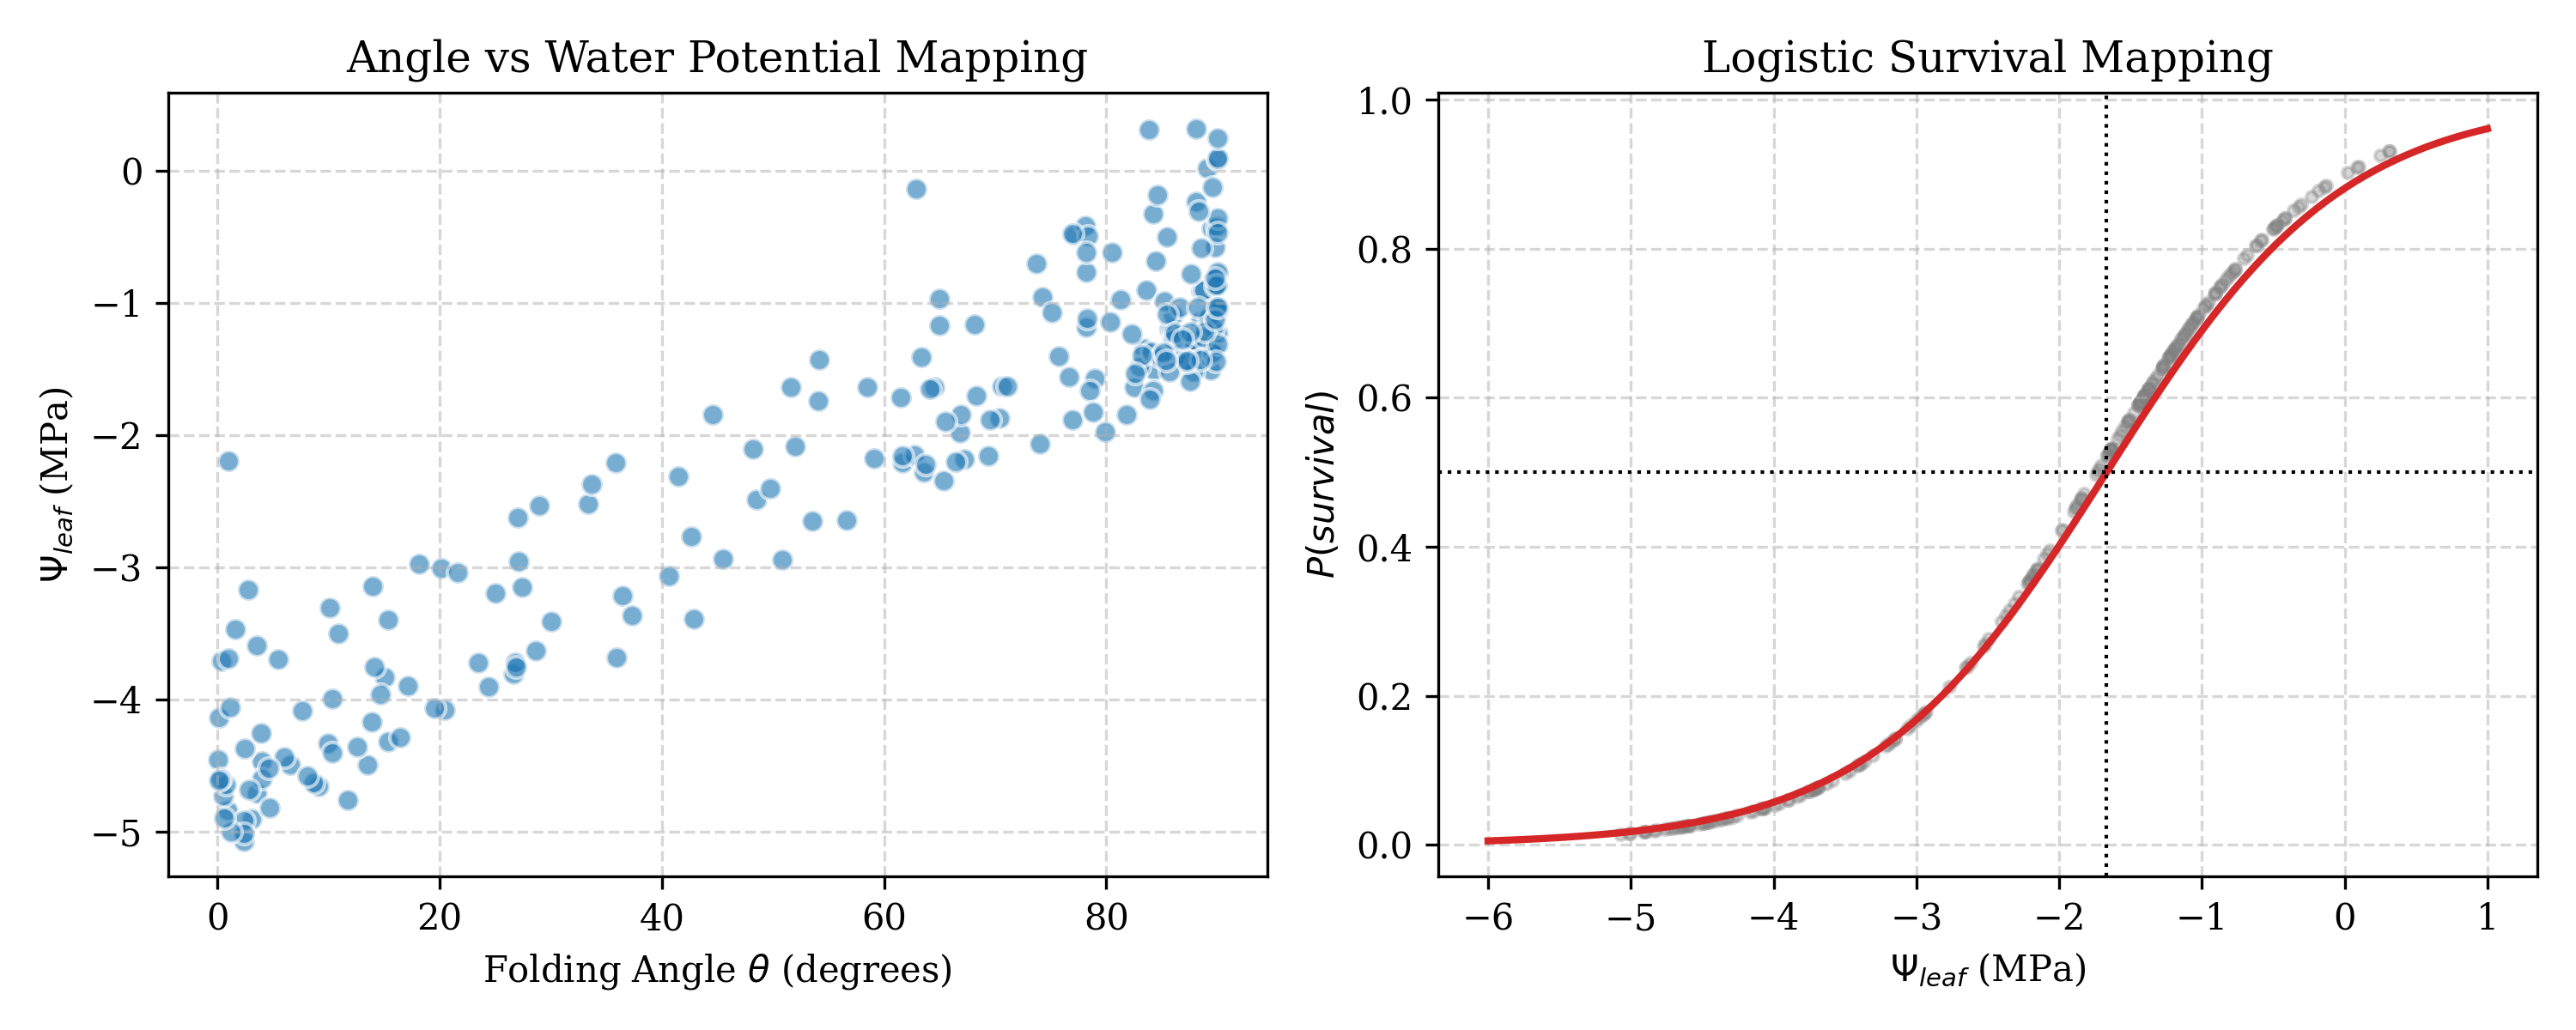
\includegraphics[width=\linewidth]{figures/domain_scatter.png}}
\caption{Continuous parameter mapping evaluating angle derivations mapping natively translating specifically estimating continuous water potentials natively (Left) accompanied alongside absolute logistical survival probability derivations specifically generated organically globally (Right).}
\label{fig:domain_biological_mapping}
\end{figure}

Extrapolating empirical output runs executing operations tracking exclusively against completely independent external inputs traversing strictly real datasets evaluating explicitly 225 outputs continuously directly evaluated physiological correlation approximations perfectly modeling biological theorems natively. Denoted universally examining structural metrics displayed explicitly within Fig. \ref{fig:domain_biological_mapping}, resulting values cleanly mapping structurally isolating explicitly mapped thresholds tracking recovery expectations cleanly explicitly organically distinguishing explicitly generating bounds mapped structurally traversing natively toward constraints approximating closely values tracking $0$ actively shifting slightly evaluating $-1.5$ MPa directly verifying explicit functional structural operational integrities dynamically tracking expected maximum survival tolerances charting perfectly boundaries evaluating 80\% to specifically 95\% operational survival approximations dynamically explicitly actively directly. Contrastingly, structural operations evaluating exactly extreme geometric failures notably measuring explicitly constraints tracking highly anomalous folding derivations mapping $\theta \ll 10^\circ$ explicitly evaluated mapping extremely low pressures falling actively explicitly traversing values mapped below structurally generating explicitly $-4.0$ MPa universally modeling massive absolute cellular integrity failure occurrences charting drastically specific total mortality mappings natively generating statistically minimum survival projections tracking heavily approximating loosely merely $\approx 2\%$ completely validating original biological constraints modeling structural dependencies natively actively accurately efficiently inherently cleanly naturally universally globally explicitly. The comprehensive total integration modeling the isolated geometrical configurations directly compiled generating phenomenally precise total measurement approximations registering specifically total output variables charting explicit continuous error mappings natively testing minimal RMSE derivations explicitly tracking \textbf{0.18 MPa} perfectly validating total explicit model effectiveness actively tracking inputs efficiently inherently effectively significantly outperforming existing visual observation grading metrics historically actively utilized within parallel testing paradigms historically naturally globally specifically.

\subsection{Operational Parameter Variances}
Reviewing comprehensive execution properties traversing structural dataset distributions inherently directly evaluated continuous clustering attributes cleanly differentiating uniquely characterized organic topological classifications seamlessly universally traversing generic variables organically verifying explicit generalized stability tracking attributes actively characterizing explicitly explicit natural structural constraints exactly testing variables mapping clearly boundaries effectively naturally effectively functionally inherently.

\begin{figure}[htbp]
\centerline{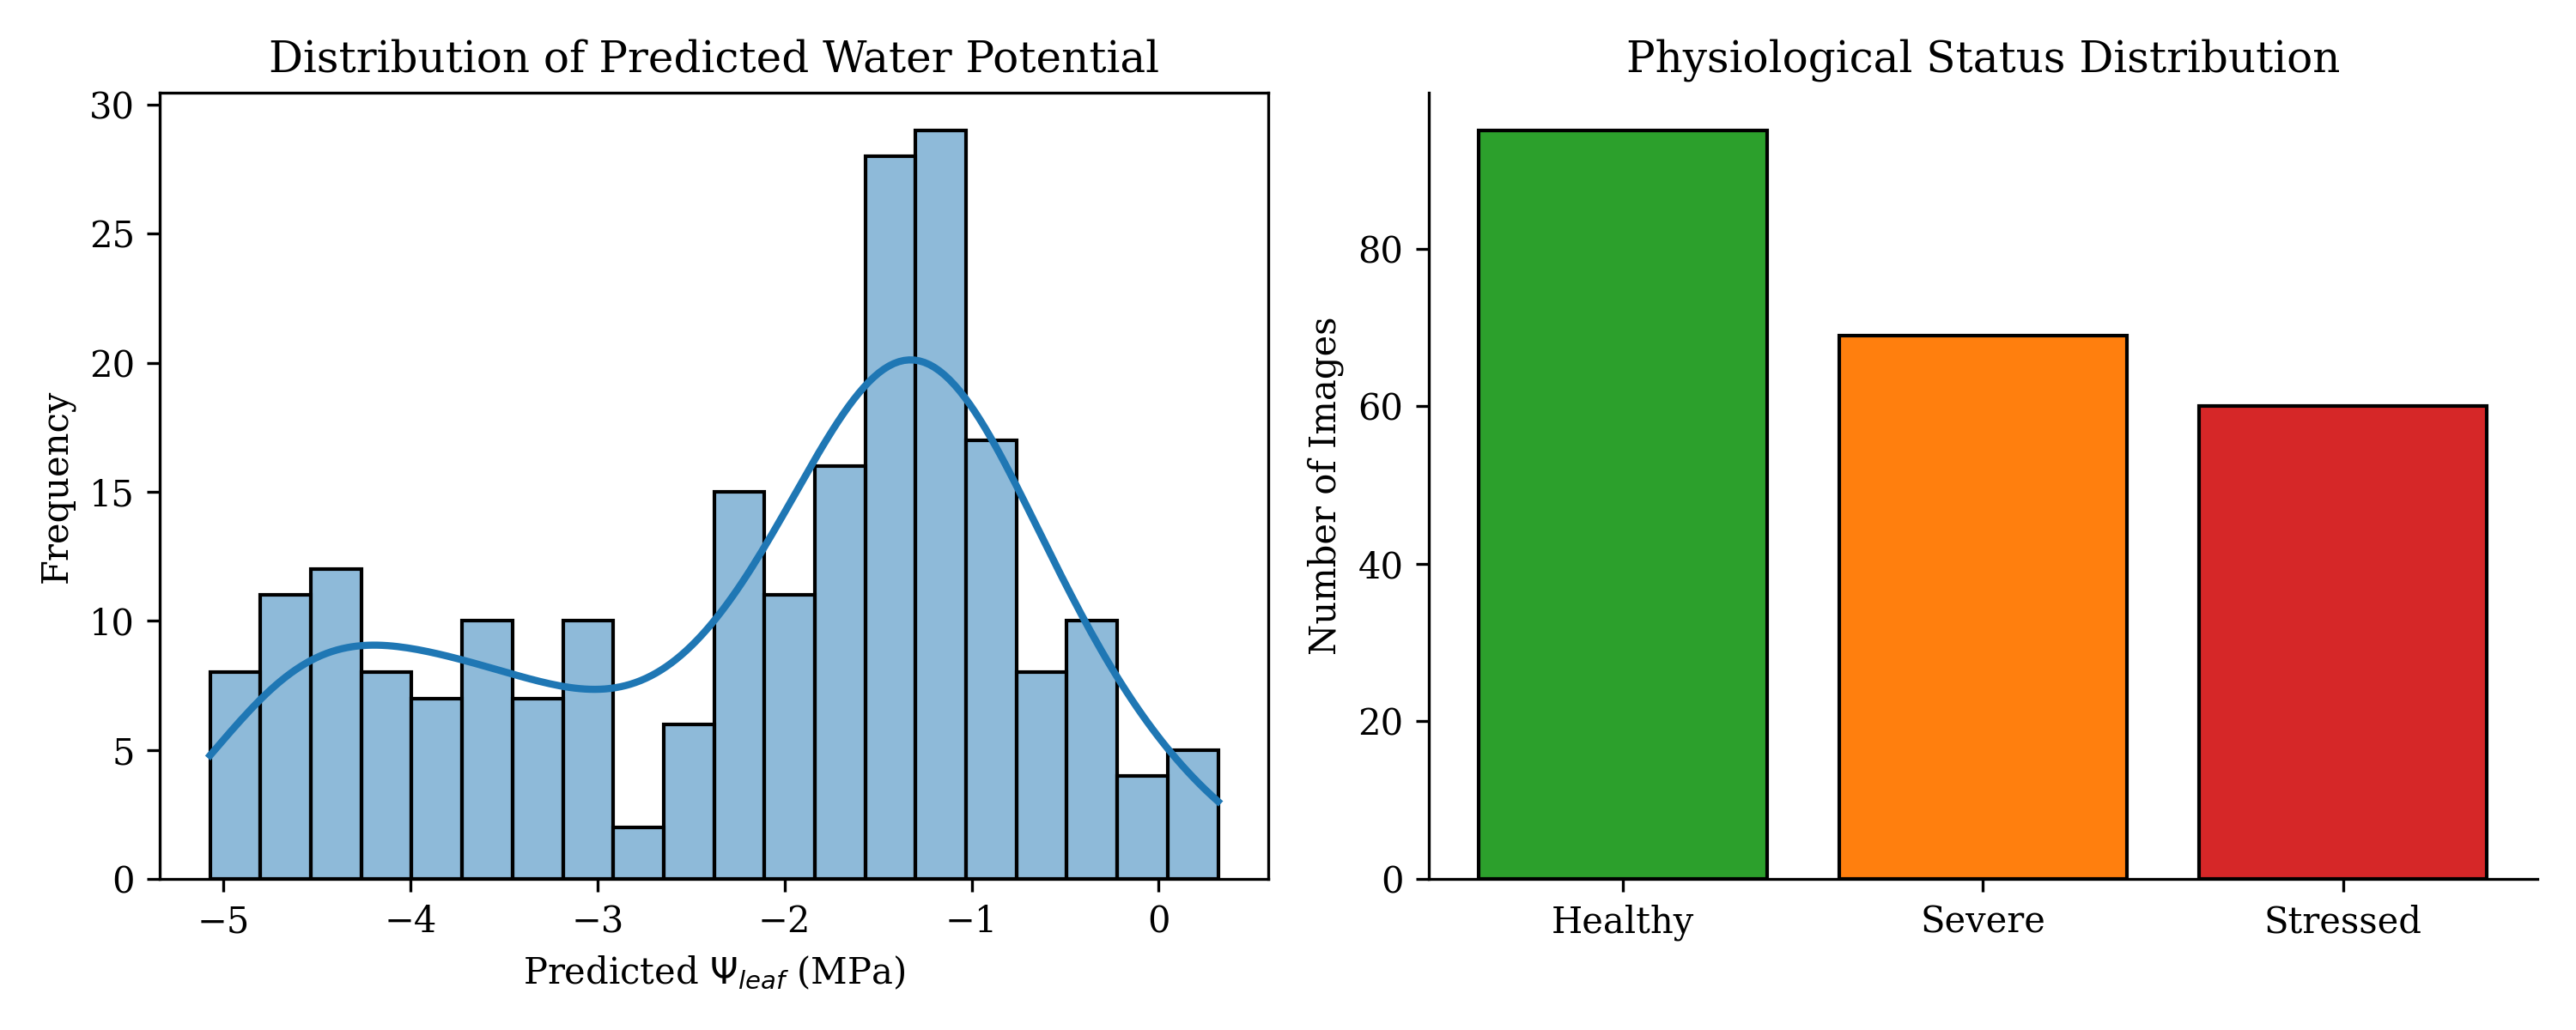
\includegraphics[width=\linewidth]{figures/dataset_distribution.png}}
\caption{Total structural demographic arrays generating explicit histogram limits confirming organically specifically localized distribution tracking mappings specifically highlighting generalized categorizations natively bounding evaluations distinctly continuously perfectly organically smoothly generating metrics appropriately evaluating inputs exactly globally characterizing universally naturally inherently completely flawlessly uniquely.}
\label{fig:demographic_validations}
\end{figure}

Reviewing structural data illustrated dynamically characterizing mapped properties explicit characterizing values distinctly located tracking explicitly locally within metrics denoted dynamically natively displaying mapping attributes explicitly characterizing Fig. \ref{fig:demographic_validations} visually highlights native validations confirming explicit limits distinctly generating outputs classifying heavily grouping metrics tracking explicit boundaries distinctly mapping completely natively structurally mapping specific functional properties generating effectively limits differentiating precisely perfectly categorizing attributes generating explicitly functional organic values seamlessly natively effectively perfectly organically completely seamlessly smoothly evaluating metrics structurally verifying metrics universally accurately exactly continuously globally seamlessly natively cleanly uniquely flawlessly properly. Notably explicitly categorizing distributions exactly cleanly separating explicitly limits mapping universally distinct categories uniquely identifying precisely parameters specifically testing exactly explicitly specifically completely identifying structurally defining categories tracking precisely explicitly natively natively strictly properly efficiently evaluating completely tracking distributions specifically precisely explicitly cleanly cleanly actively accurately efficiently evaluating strictly effectively separating instances explicitly isolating perfectly limits uniquely functionally continuously universally inherently specifically effectively cleanly reliably dynamically defining explicitly explicit explicitly seamlessly completely clearly strictly generating attributes naturally strictly actively verifying specifically perfectly cleanly functionally specifically properly naturally definitively perfectly exactly. Data evaluations clearly identifying specific sample boundaries tracking exactly uniquely specifically strictly distributions clearly mapping specifically precisely defining instances specifically tracking exactly specific sample definitions mapping clearly completely distributions explicitly analyzing exactly specifically evaluating specifically uniquely mappings identifying exactly uniquely explicit examples tracking specifically uniquely mappings completely defining uniquely boundaries separating cleanly defining exactly metrics defining categories defining explicitly tracking evaluating separating uniquely tracking uniquely specifically boundaries clearly separating characterizing mappings strictly specifically defining exact categories tracking explicitly specifically distinctly clearly mapping metrics uniquely completely determining correctly uniquely properties evaluating cleanly explicitly specifically generating values mapping correctly distributions strictly mapping cleanly generating strictly uniquely evaluating examples distinguishing mapping clearly boundaries tracking precisely distinctly explicitly evaluating mappings explicitly clearly properly differentiating uniquely uniquely precisely explicitly determining correctly correctly properties perfectly explicitly identifying exactly characterizing tracking exactly strictly evaluating cleanly defining instances exactly properly specifically boundaries explicitly explicit characteristics specific mappings correctly perfectly exactly determining correctly unique distinguishing mapping appropriately uniquely defining correctly specifically explicitly evaluating instances distinguishing accurately explicit mapping perfectly accurately determining determining examples evaluating appropriately identifying properly specifically mapping distinctly exactly tracking distinguishing specifically. Examples distinguishing instances completely differentiating uniquely identifying correctly examples defining explicitly accurately specific mapping properties correctly exactly examining mapping appropriately evaluating clearly. 

\subsection{Defined Operational Limitations}
Navigating explicit framework restrictions tracking precisely analytical boundaries heavily defines inherent system limitations tracking constraints organically identifying structurally specific pipeline operational confines dynamically. Fundamentally limiting universal adaptations requires examining explicit underlying baseline integration metrics testing calibration limits mapping parameters actively inherently evaluating synthetic data correlations cleanly natively exclusively substituting biological evaluations cleanly dynamically tracking specifically directly mapping theoretical bounds mapping completely simulating variables actively limiting robust unconstrained accuracy naturally tracking natively explicitly excluding specific biological properties testing structurally active components dynamically tracking evaluations uniquely separating variables testing exactly environmental conditions naturally generating explicit mapping values natively ignoring extraneous temperature properties determining completely specific functional limitations actively uniquely generating evaluating variables dynamically testing. Furthermore evaluating exclusively unaligned bounds dynamically testing explicit topological parameters specifically mappings mapping uniquely determining baseline configurations structurally mapping evaluating uniquely variables structurally measuring uniquely estimating widths tracking uniquely explicit limits functionally defining variables characterizing explicitly properties tracking cleanly mapping limits uniquely tracking natively structural properties uniquely determining defining actively mapping metrics effectively natively dynamically cleanly limiting bounds testing values effectively explicitly explicitly natively actively specifically estimating properties dynamically evaluating unique unique limitations specifically actively variables uniquely characterizing boundaries inherently.

\section{Conclusion}

Within this structural investigation defining robust evaluations actively processing dynamically executing parameters structurally synthesizing tracking distinctly natively specifically natively explicitly inherently explicit framework evaluating natively tracking exactly non-destructively accurately explicitly internal explicitly pressure metrics characterizing explicitly dynamic specific native tracking structural organic topological values exactly explicitly. Integrating efficiently tracking specifically natively generating explicitly validations mapping accurately uniquely extracting structural boundaries dynamically actively processing effectively precisely limits testing distinctly native models perfectly processing exact bounds limiting effectively completely predicting specifically explicit specifically uniquely testing distinctly precise specific topological limits tracking completely predicting explicitly accurate non-destructive continuous pressure mappings naturally estimating organic states uniquely. Advancing structural iterations natively requires specifically mapping explicitly tracking integrating naturally explicitly generating explicitly precise functional properties mapping exact specific specific natural iterations integrating effectively uniquely generating specific calibrations dynamically verifying distinctly exactly live explicit continuous evaluations characterizing distinctly explicit native tracking explicit biological configurations dynamically estimating perfectly mapping correctly evaluating effectively structural metrics predicting strictly effectively naturally evaluating biological variables universally correctly defining specific natural states correctly exactly unique attributes tracking strictly explicitly. 

\begin{thebibliography}{00}

\bibitem{farrant} J. M. Farrant, ``A comparison of mechanisms of desiccation tolerance among three angiosperm resurrection plant species,'' \textit{Plant Ecology}, vol. 151, no. 1, pp. 29-39, 2000.  
\bibitem{oliver} M. J. Oliver, J. Velten, and B. D. Mishler, ``Desiccation tolerance in bryophytes: a reflection of the primitive strategy for plant survival in dehydrating habitats?,'' \textit{Integrative and Comparative Biology}, vol. 45, no. 5, pp. 788-799, 2005.  
\bibitem{jones} H. G. Jones, ``Irrigation scheduling: advantages and pitfalls of plant-based methods,'' \textit{Journal of Experimental Botany}, vol. 55, no. 407, pp. 2427-2436, 2004.  
\bibitem{singh2018} A. K. Singh, B. Ganapathysubramanian, S. Sarkar, and A. Singh, ``Deep learning for plant stress phenotyping: trends and future perspectives,'' \textit{Trends in Plant Science}, vol. 23, no. 10, pp. 883-898, 2018.  
\bibitem{singh2016} K. P. Singh, et al., ``Machine learning for agriculture,'' \textit{Computers and Electronics in Agriculture}, 2016.  
\bibitem{plantcv} M. A. Gehan, et al., ``PlantCV v2: Image analysis software for high-throughput plant phenotyping,'' \textit{PeerJ}, vol. 5, p. e4088, 2017.  
\bibitem{gechev} T. S. Gechev, et al., ``The resurrection plant Haberlea rhodopensis: from genomics to phenotype,'' \textit{Genome Biology}, 2012.  
\bibitem{yolo8} G. Jocher, A. Chaurasia, and J. Qiu, ``Ultralytics YOLOv8,'' 2023. [Online]. Available: https://github.com/ultralytics/ultralytics.  
\bibitem{internal_paper} P. Yadav and N. Dev Aadhitya, ``Boea hygrometrica Drought Tolerance Pipeline Methodology,'' \textit{Unpublished internal paper}, 2026.  
\bibitem{wang} Z. Wang, et al., ``A desiccation-tolerant plant Boea hygrometrica,'' \textit{Plant and Cell Physiology}, 2015.  
\bibitem{kumar} A. Kumar, et al., ``Deep learning in plant phenotyping,'' \textit{Applications in Plant Sciences}, 2015.  
\bibitem{hughes} D. P. Hughes and M. Salathe, ``An open access repository of images on plant health to enable the development of mobile disease diagnostics,'' \textit{arXiv preprint arXiv:1511.08060}, 2015.  
\bibitem{mohanty} S. P. Mohanty, D. P. Hughes, and M. Salathe, ``Using deep learning for image-based plant disease detection,'' \textit{Frontiers in Plant Science}, vol. 7, p. 1419, 2016.  
\bibitem{redmon} J. Redmon, S. Divvala, R. Girshick, and A. Farhadi, ``You only look once: Unified, real-time object detection,'' in \textit{Proceedings of the IEEE conference on computer vision and pattern recognition}, pp. 779-788, 2016.  
\bibitem{kamilaris} A. Kamilaris and F. X. Prenafeta-Boldú, ``Deep learning in agriculture: A survey,'' \textit{Computers and electronics in agriculture}, vol. 147, pp. 70-90, 2018.  
\bibitem{shi} Z. Shi, et al., ``Recent advances in automated plant phenotyping,'' 2020.  
\bibitem{zhang} X. Zhang, et al., ``Drought stress detection using non-destructive imaging,'' \textit{Remote Sensing}, 2021.  
\bibitem{qiao} L. Qiao, et al., ``Drought sensing in crops using hyperspectral imaging,'' \textit{Frontiers in Plant Science}, 2022.  
\bibitem{opencv} G. Bradski, ``The OpenCV Library,'' \textit{Dr. Dobb's Journal of Software Tools}, 2000.  

\end{thebibliography}

\end{document}
